\section{Parallel Algorithms}
\subsection{Parallel Programming}
%%%%%%%%%%%%%%%%%%%%%%%%%%%%%%%%%%%%%%%%%%%%%%%%%%%%%%%%%%%%%%%%%%%%%
%\royslide{Parallel:: API}{
\begin{frame}[fragile]
\frametitle{Parallel:: API}
\royitemizebegin{Encapsulating MPI}
\item Improvement over MPI C++ interface
\item Makes code shorter, more legible
\royitemizeend

Example:
\small
\begin{semiverbatim}
std::vector<Real> send, recv;
...
send\_receive(dest\_processor\_id, send,
             source\_processor\_id, recv);
\end{semiverbatim}
\end{frame}
%}



%%%%%%%%%%%%%%%%%%%%%%%%%%%%%%%%%%%%%%%%%%%%%%%%%%%%%%%%%%%%%%%%%%%%%
%\royslide{Parallel:: API}{
\begin{frame}[fragile]
\frametitle{Parallel:: API}

Instead of:
\tiny
\begin{semiverbatim}
if (dest\_processor\_id   == libMesh::processor\_id() \&\&
    source\_processor\_id == libMesh::processor\_id())
  recv = send;
#ifdef HAVE\_MPI
else
  \{
    unsigned int sendsize = send.size(), recvsize;
    MPI\_Status status;
    MPI\_Sendrecv(\&sendsize, 1, datatype<unsigned int>(),
                 dest\_processor\_id, 0,
                 \&recvsize, 1, datatype<unsigned int>(),
                 source\_processor\_id, 0,
                 libMesh::COMM\_WORLD,
                 \&status);

    recv.resize(recvsize);

    MPI\_Sendrecv(sendsize ? \&send[0] : NULL, sendsize, MPI\_DOUBLE,
                 dest\_processor\_id, 0,
                 recvsize ? \&recv[0] : NULL, recvsize, MPI\_DOUBLE,
                 source\_processor\_id, 0,
                 libMesh::COMM\_WORLD,
                 \&status);
  \}
#endif // HAVE\_MPI
\end{semiverbatim}
\end{frame}
%}


%%%%%%%%%%%%%%%%%%%%%%%%%%%%%%%%%%%%%%%%%%%%%%%%%%%%%%%%%%%%%%%%%%%%%
\royslide{ParallelMesh Data Structure}{
\royitemizebegin{std::vector fails}
\item Not sparse
\item $O(N_E)$ storage cost
\royitemizeend
\royitemizebegin{std::map}
\item ``mapvector'' interface provides iterators
\item $O(log (N_E/N_P))$ lookup time without std::hash\_map
\item $O(1)$ lookup time with std::hash\_map
\royitemizeend
\royitemizebegin{Hybrid data structure?}
\item Dense vector for most elements
\item Sparse data structure for new elements
\royitemizeend
}



\subsection{Inter-Processor Communication}
%%%%%%%%%%%%%%%%%%%%%%%%%%%%%%%%%%%%%%%%%%%%%%%%%%%%%%%%%%%%%%%%%%%%%
\royslide{Round Robin Communications}{

\begin{columns}
\begin{column}{.5\textwidth}
\begin{center}
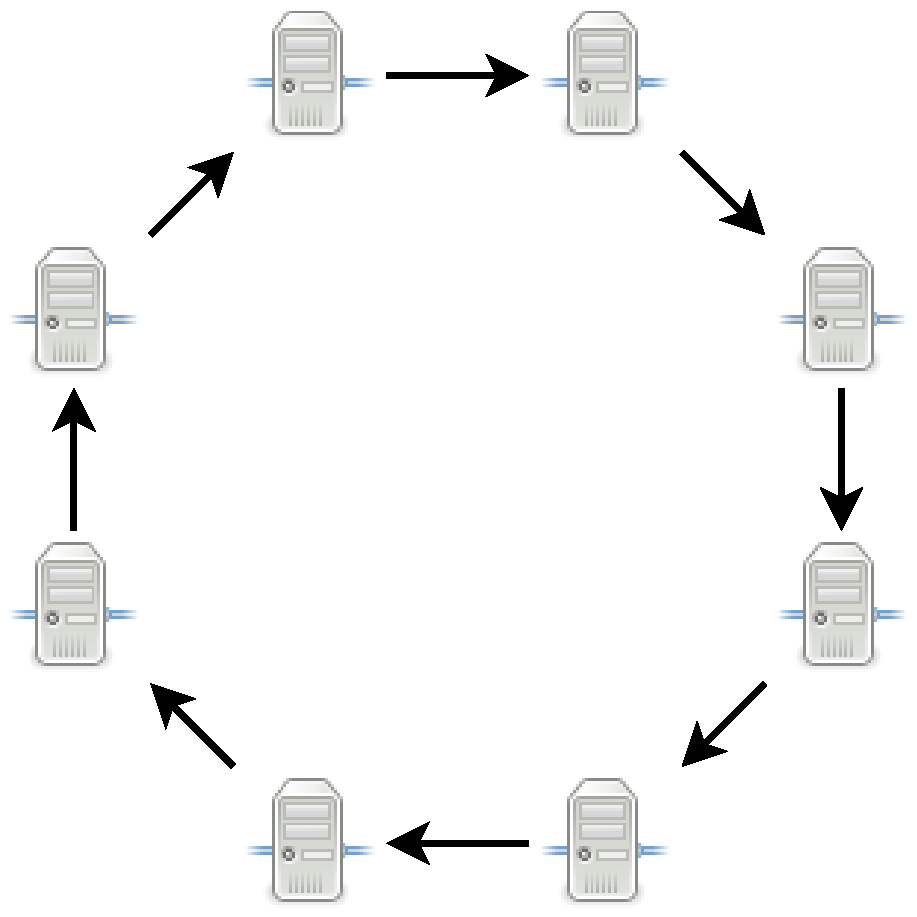
\includegraphics[width=.9\textwidth]{figs/RoundRobin1}
\end{center}
\end{column}
\begin{column}{.5\textwidth}
\royitemizebegin{}
\item Processor $P$ sends to processor $P+K$ while receiving from $P-K$
\item New data is operated on and old data discarded
\item $K$ is incremented ``round robin'' from $1$ to $N_P-1$
\royitemizeend
\end{column}
\end{columns}
}



%%%%%%%%%%%%%%%%%%%%%%%%%%%%%%%%%%%%%%%%%%%%%%%%%%%%%%%%%%%%%%%%%%%%%
\royslide{Round Robin Communications}{

\begin{columns}
\begin{column}{.5\textwidth}
\begin{center}
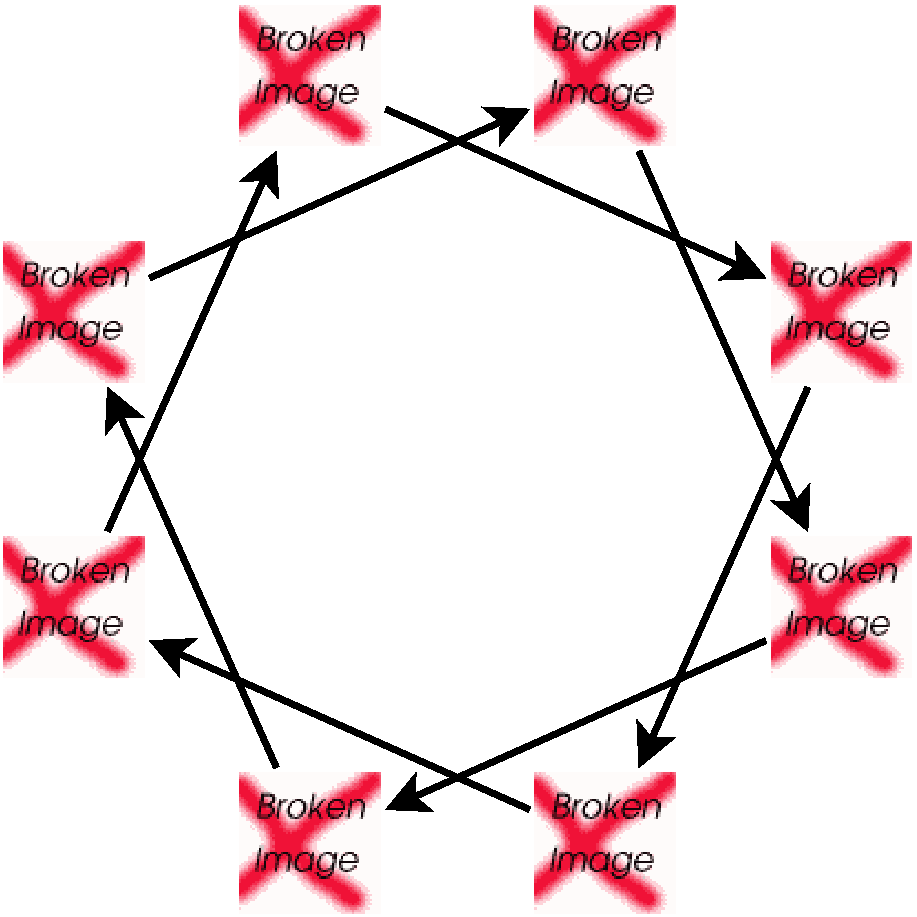
\includegraphics[width=.9\textwidth]{figs/RoundRobin2}
\end{center}
\end{column}
\begin{column}{.5\textwidth}
\royitemizebegin{Pros}
\item $O(N_G/N_P)$ memory usage - only one data exchange at a time
\item Straightforward to code
\item Reliable
\royitemizeend
\end{column}
\end{columns}
}



%%%%%%%%%%%%%%%%%%%%%%%%%%%%%%%%%%%%%%%%%%%%%%%%%%%%%%%%%%%%%%%%%%%%%
\royslide{Round Robin Communications}{

\begin{columns}
\begin{column}{.5\textwidth}
\royitemizebegin{Cons}
\item Communications loop over non-neighboring processors
\item $O(N_G)$ execution time
\item Multiple, synchronous communications
\royitemizeend
\end{column}
\begin{column}{.5\textwidth}
\begin{center}
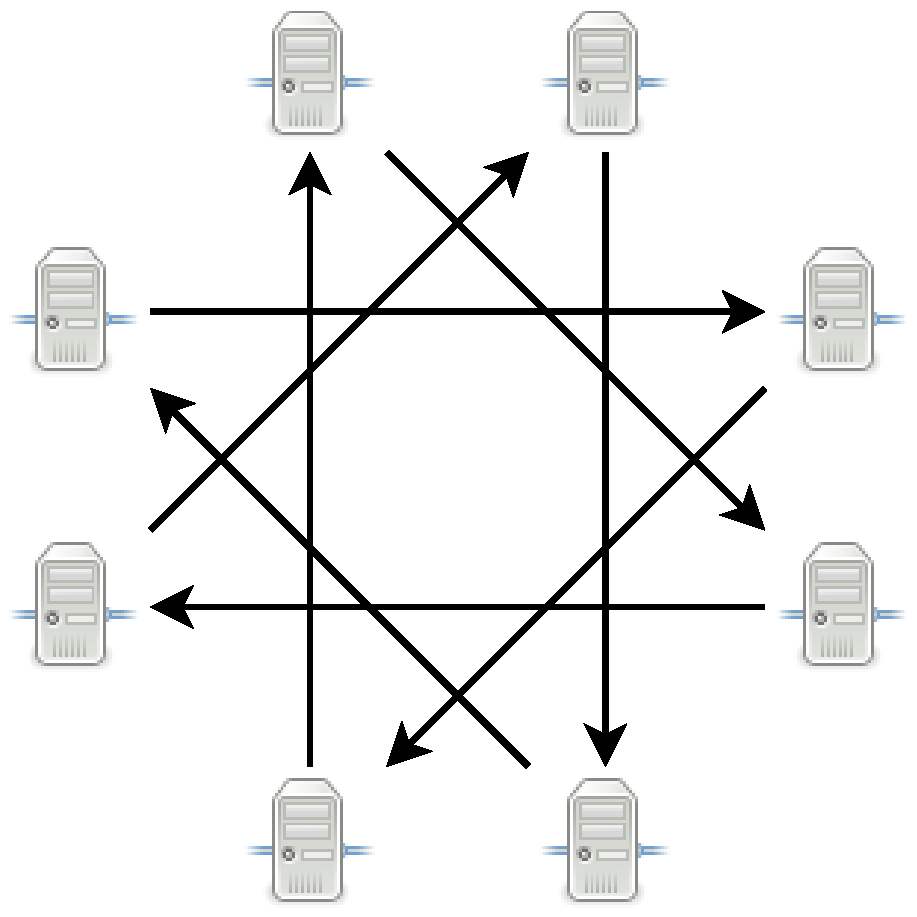
\includegraphics[width=.9\textwidth]{figs/RoundRobin3}
\end{center}
\end{column}
\end{columns}
}



\subsection{Adaptivity Issues}
%%%%%%%%%%%%%%%%%%%%%%%%%%%%%%%%%%%%%%%%%%%%%%%%%%%%%%%%%%%%%%%%%%%%%
\royslide{Adaptivity and ParallelMesh}{
\begin{columns}
\begin{column}{.5\textwidth}
\begin{center}
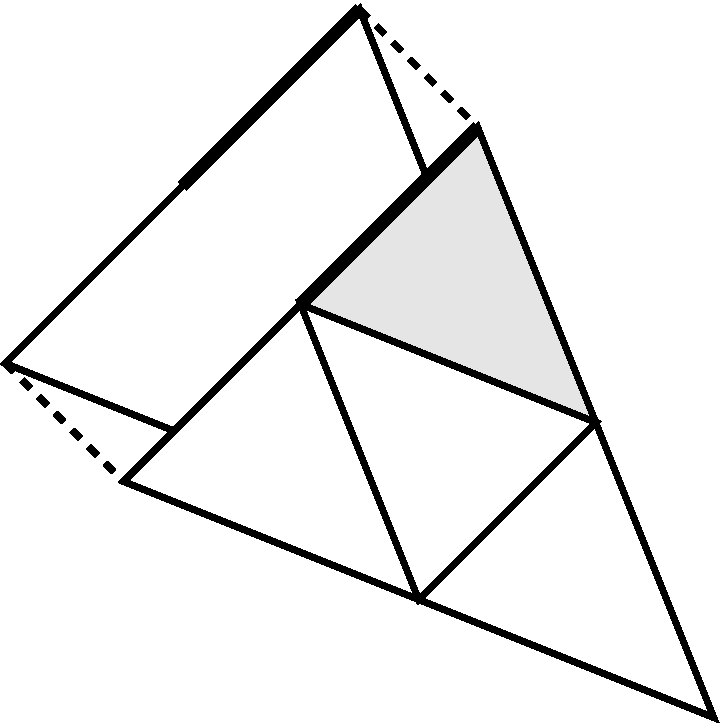
\includegraphics[width=.9\textwidth]{figs/adaptive}
\end{center}
\end{column}
\begin{column}{.5\textwidth}
\royitemizebegin{Challenges}
\item Reindexing elements, nodes, DoFs
\item Synchronization of ghost objects
\item Load balancing, Repartitioning
\royitemizeend
\end{column}
\end{columns}
}



%%%%%%%%%%%%%%%%%%%%%%%%%%%%%%%%%%%%%%%%%%%%%%%%%%%%%%%%%%%%%%%%%%%%%
\royslide{Parallel Global Indexing}{
\royitemizebegin{One-pass indexing}
\item Index processor $P$ from $\sum_1^{P-1} N_{E_p}$
\item Pass $\sum_1^P N_{E_p}$ to processor $P+1$
\item $O(N_E)$ work
\item $O(N_E)$ execution time
\royitemizeend
}



%%%%%%%%%%%%%%%%%%%%%%%%%%%%%%%%%%%%%%%%%%%%%%%%%%%%%%%%%%%%%%%%%%%%%
\royslide{Parallel Global Indexing}{
\royitemizebegin{Two-pass indexing}
\item Count processor $P$ indices from 0
\item Gather $N_{E_p}$ on all processors
\item Re-index processor $P$ from $\sum_1^{P-1} N_{E_p}$
\item Double the work
\item $O(N_E/N_P)$ execution time
\royitemizeend
}



%%%%%%%%%%%%%%%%%%%%%%%%%%%%%%%%%%%%%%%%%%%%%%%%%%%%%%%%%%%%%%%%%%%%%
\royslide{Parallel Synchronization}{
\royitemizebegin{What can lose sync?}
\item Refinement flags
\item New child elements, nodes
\item New degrees of freedom
\item Hanging node constraint equations
\item Repartitioned elements, nodes
\royitemizeend
}



%%%%%%%%%%%%%%%%%%%%%%%%%%%%%%%%%%%%%%%%%%%%%%%%%%%%%%%%%%%%%%%%%%%%%
\royslide{Parallel Synchronization}{
\royitemizebegin{Round-Robin Complications}
\item Refinement flags must obey consistency rules
\item New ghost nodes may have unknown processor ids
\item Constraint equations may be recursive
\item Hanging node constraint equations
\item Repartitioned elements, nodes
\royitemizeend
}
